\documentclass[12pt]{article}

\usepackage{graphicx}
\graphicspath{{figures/}}

\textheight=210mm
\textwidth=155mm

\hoffset=-1mm
\voffset=-10mm

\usepackage{color}
\def\bb{\begin{color}{blue}}
\def\br{\begin{color}{red}}
\def\eb{\end{color}\ }

\begin{document}

\begin{center}
{\bf Response to Reviewer A's comments}\\
on paper `` A novel scaling indicator of early warning signals 
helps anticipate tropical cyclones ''\\[5pt]
by {\it J.~Prettyman, T.~Kuna, and V.~N.~Livina}
\end{center}

\vspace{3mm}

\noindent We would like to thank the Reviewer for the positive
opinion about the novel indicator. We have revised the paper according to 
the reviewer's comments as follows.

\begin{itemize}
\item[\bf Comment 1.] 
{\sl
The paper follows ideas proposed by Scheffer et al. (ref. 6), 
which uses the well-known fact that in the special case of a 
system represented by a variable x(t) approaching a saddle-node 
bifurcation, the auto-correlation of x(t) will increase prior 
to the bifurcation (critical slow down) as $t \rightarrow t_c$. 
[...] Obviosly, 
since the power spectrum is the Fourier transform of the auto correlation 
and, in case of a scaling signal, the scaling exponents are 
directly related to the DFA exponent (eq. 4) this can be done.
[...] For this to be useful the relevant 
issue is to establish under which circumstances the proposed PS 
indicator is better or worse than the other EWS indicators. 
This discussion is completely lacking. }

\item[\bf Response.] 
The aim of this paper is not to investigate analytically in which 
dynamical systems the PS-indicator would be better or worse than other 
EWS methods, but rather to show that, in principle, the PS-indicator 
may provide an EWS. This is done by comparison to the ACF(1) and 
DFA indicators - not to show that it is better or worse, but simply 
to show that it behaves similarly, which in theory it should 
(as is pointed out by the reviewer, above). 
A comment to this effect has been added to the introduction.

We would like to note that the present manuscript follows the ideas 
of the paper [Livina and Lenton, GRL 2007] rather than the later paper 
mentioned by the reviewer [Scheffer et al, 2009].

\item[\bf Comment 2.]
{\sl 
Nn the case(s) where we have a theoretical foundation for 
how the EWS indicators behave (simple bifurcations), 
the question of length and resolution of the time series at 
hand in relation to estimating the different measures should be discussed. 
From figure 3 it is apparent that PS is useless as EWS for the 
pitchfork bifurcation, DFA is marginal and only ACF(1) can be used. 
This is because in order to avoid false positives at the 1sigma level 
(very low, should be at least 2sigma), the mean should be outside 
the 1sigma level (gray band in fig 3). 
That does not happen for PS before t=600.  
}

\item[\bf Response.] 
The reviewer is right that length and resolution of the series are 
important aspects of time series analysis. 

In the case of high-frequency sampling
of data, it is likely that the autocorrelation would be fluctuating 
at very high level (close to maximal value~1) and not providing any 
meaningful EWS information. In such cases, for applying any EWS indicator
based on scaling properties (ACF, DFA or PS), it would be useful to 
pre-process the data with 
some aggregation or averaging, similarly to~\cite{held2004}. 
However, this issue is not specific to the 
new PS-indicator. Moreover, in many cases a time series is pre-processed 
before calculating EWS indicators (for instance, using Gaussian filter
or moving average), which immediately changes the absolute value of
autocorrelation and other scaling exponents. This means that the critical 
value of autocorrelation changes, and it is no longer bounded 
by the critical
value~1. In such cases, the increasing trend of an EWS indicator is more
informative than its values, which is a shortcoming of the approach with 
such data pre-processing. So far, its impact on the EWS 
indicators has not been studied, either in the context of analytical 
rigour or in the context of proximity to a tipping point; 
this must be a topic of further research in the area of 
early warning signals.

On the other hand, the length of the series (always
finite and often imposing finite-size-effect challenges) may be problematic
in case of estimation, for instance, variance in fixed-size windows. 
As was demonstrated in Fig.2 (middle panel) 
of~\cite{livina2012}, using
fixed-size window in studying a dataset with increasing scaling exponent 
may generate a decreasing variance indicator. 

We have added this text in the Discussion section. 

We have included a short discussion about the 
PS-indicator applied to the pitchfork bifurcation (figure 3), 
drawing attention to the fact that the mean does not rise above 
the 1sigma level.

\item[\bf Comment 3.]
{\sl 
The simulation (eq. 6) is fine, and I think the right way of testing. 
It is identical to what we presented in (Ditlevsen and Johnsen, GRL 2010) 
in the generic saddle node bifurcation case. In this connection 
the authors should argue why they omit using the increased variance,
which we demonstrate is the strongest EWS indicator.
The authors may want to look at: (Peter D. Ditlevsen, 
``Tipping Points in the Climate System'', to appear in 
``Nonlinear and Stochastic Climate Dynamics'' 
(Ed. Christian Franzke and Terence O'Kane), Cambridge Univ. Press, 2017).
}

\item[\bf Response.] 
We thank the reviewer for the reference to (Peter D. Ditlevsen, 
``Tipping Points in the Climate System'', 2017), and 
we have added it to our bibliography.

We considered only ACF(1) 
(as a proxy for the auto correlation scaling exponent) and DFA, 
besides the novel power spectrum (PS) indicator because the 
inspiration came from [Kantelhardt et al. 2001], which provides 
a relationship between these three scaling exponents, and because 
the paper was considered a natural progression from 
[Livina and Lenton, GRL, 2007] where the DFA propagator was 
introduced.
As was mentioned in the response to Comment 2, in some cases of changing
scaling properties, the variance indicator may decrease prior to a 
bifurcation, as was demonstrated on artificial data studied with a 
fixed-size window.

\item[\bf Comment 4.]
{\sl 
Beside the few generic cases of bifurcations, for other 
tipping points or critical transitions the statistical quantities 
behave differently. The idea of change in long-range correlations 
comes from phase transitions in statistical mechanics. 
Here the transitions are usually characterized by emergence of 
long range correlations (power law behaviour), from the disordered 
state with short range (exponential) correlations and not by change 
of a scaling exponent. Actually the main characteristic of these 
critical transitions is the uniqueness (universality) of the scaling 
exponents. This should be discussed much more rigorously, 
especially also when a geophysical fluid dynamical situation as 
passing of cyclones is analysed. What type of dynamics is this, 
and what kind of EWS should we expect?
}

\item[\bf Response.]
The pitchfork bifurcation is chosen as an example of a system where we 
will definitely expect the ACF(1) indicator to provide a very good EWS, 
therefore allowing us to see the new indicator applied to a familiar system. 
The approaching cyclone is chosen as an example of a system which 
has not previously been studied using these tipping-point 
EWS methods, and for which the dynamics of the system are unknown, 
thus providing a "blind" experiment. The passing cyclone is not 
modelled as a phase transition, and it is not known whether 
there exists a critical point such that we might claim universality 
of the scaling exponents. Rather, we have a time series which 
superficially resembles other geophysical tipping-point examples 
(such as in [Dakos et al. {\it Slowing down as an early warning 
signal for abrupt climate change}, PNAS, 2008]), thus we wish to 
experiment with our existing EWS methods, and then compare the 
performance of our new indicator. In this sense, it is an heuristic investigation of the properties of the new technique, with 
comparison with similar methods. We report our findings to facilitate
further investigation of this technique.

We have added this text into the manuscript. 


\item[\bf Comment 5.] 
{\sl 
What does ``scaling properties similar to ACF'' mean? 
In the standard cases (including eq. 6) the ACF is exponential, 
and the PS has two scaling regimes beta=0 and beta=2. This means 
that the PS indicator related to critical slow down is beta 
increasing from -2 to 0.
}

\item[\bf Response.]
In the phrase ``Since DFA provides a method to study the 
scaling properties, similarly to the ACF, the DFA scaling indicator 
has been introduced...'', we are making the point that the DFA 
indicator provides a method to study longer-range 
scaling properties when they can be estimated, and 
in this respect it is similar to ACF. This is applicable to 
the changing scaling during the critical slow-down, when 
ACF ceases to decay exponentially and demonstrates scaling properties,
similarly to DFA and PS. To clarify this, we added a note on 
slowing down in the same sentence. 
%%%{\bb What is meant by ``two scaling regimes beta=0 and..''???\eb}

\item[\bf Comment 6.] %%% DONE
{\sl 
Abstract: Define ``critical mode''. 2 lines after eq. 1: 
``uncorrelated'' should be ``short range correlated''. 
}

\item[\bf Response.]
We have changed the manuscript to accommodate the suggestions 
(critical modes, short-range correlated).

\item[\bf Comment 7.]
{\sl 
How are data in Fig 1 generated? (I guess it is similar to Fig 2).
}

\item[\bf Response.]
The data in fig.1 are indeed generated similarly to fig.2, 
we have added a note on this in the revised manuscript.

\item[\bf Comment 8.]
{\sl 
Eq.5: I would have preferred something like a fractional 
Brownian motion (fBm) or some other less artificial standard process 
(and a discussion of why the usual Ornstein-Uhlenbeck red noise process 
is not relevant).
}

\item[\bf Response.]
We have chosen this artificial time series, rather than the 
Ornstein-Uhlenbeck process, to reflect the result in 
[Livina et al 2012] 
and to provide an example specifically suited to the PS-indicator. 
A note of this has been included in the manuscript.

\item[\bf Comment 9.]
{\sl 
Eq. 6: It should be discussed why the pitchfork bifurcation 
is studied rather than the generic saddle node. Pitchfork is special: 
It requires a perfect symmetry (and turns into saddle node with any 
small symmetry breaking perturbation). In perfectly symmetric systems, 
we often know more about the dynamics such that bifurcations can be 
predicted more precisely than what can be done with EWS.
}

\item[\bf Response.] 
The pitchfork bifurcation was chosen because in this case
ACF(1) provides a clear EWS. Therefore, it is a good testbed for the PS-indicator, by analogy.  

We have included here a similar experiment using a saddle node bifurcation described by the stochastic differential equation 
\begin{equation} 
\dot{z}(t) = -\frac{\partial}{\partial z}\left(\frac{z^4}{4} - \frac{z^2}{2} - \left(0.003t - 2\right)z\right) + \sigma\eta_t, 
\label{saddlenode_eqn} 
\end{equation} 
where $\sigma=0.2$ and the $\eta_t$ are independent samples from a Gaussian distribution. Equation \ref{saddlenode_eqn} is integrated numerically with a time step of $\delta t$ = 0.05 from $t=1$ to $t=1000$, and sampled with $\Delta t = 1$. In the range $t<795$ the system has only one stable node in the region $z<0$, at $t\approx 540$ the the system becomes a double well with another stable node in the region $z>0$, but the noise is small enough that the system does not jump between stable nodes. The system then bifurcates after at $t\approx 795$ when the first stable node disappears, forcing the system to roll into the new stable state.

The system is integrated 50 times to produce 50 time series of length 1000, see fig. \ref{fig_new}a. The EWS indicators are then applied to the 50 time series and the mean of all 50 indicator series is plotted with error bars of one standard deviation. We have performed this with the ACF(1)- and DFA-indicators (fig.~\ref{fig_new}b,c) and the new PS-indicator (fig.~\ref{fig_new}d). The ACF(1)-indicator provides a clear EWS as expected, there is a definite increasing trend starting at around $t=750$.

We see that the result is similar to figure 3 in the manuscript, with ACF(1) giving the clearest EWS, and all three indicators rising (to some extent) before the event time $t=795$, and the PS-indicator has a very large variance. However, it appears that the rise in all indicators can be explained by the fact that the system often jumps to the other stable node before the genuine bifurcation occurs. With $\sigma>0.2$ this effect is obviously greater. With smaller values of $\sigma$ we can be sure that the jump is not purely noise driven, since for very small $\sigma$ the jump does not occur until the exact moment of the bifurcation, but in this case it is clearly very difficult to detect any warning signal. With the pitchfork bifurcation we avoid this problem of distinguishing bifurcation-driven and noise-driven jumps because the ``other'' stable state does not exist until the bifurcation. We therefore prefer it for this specific task of comparing indicator performance (without a view to claiming that any is better or worse than another).

\end{itemize}

\vspace{7mm}

\noindent
We hope that the revised manuscript is now suitable for publication in EPL.

\vspace{5mm}

\noindent
Yours sincerely,

\vspace{1mm}

\noindent
J.~Prettyman, T.~Kuna, and V.~N.~Livina


\begin{figure}
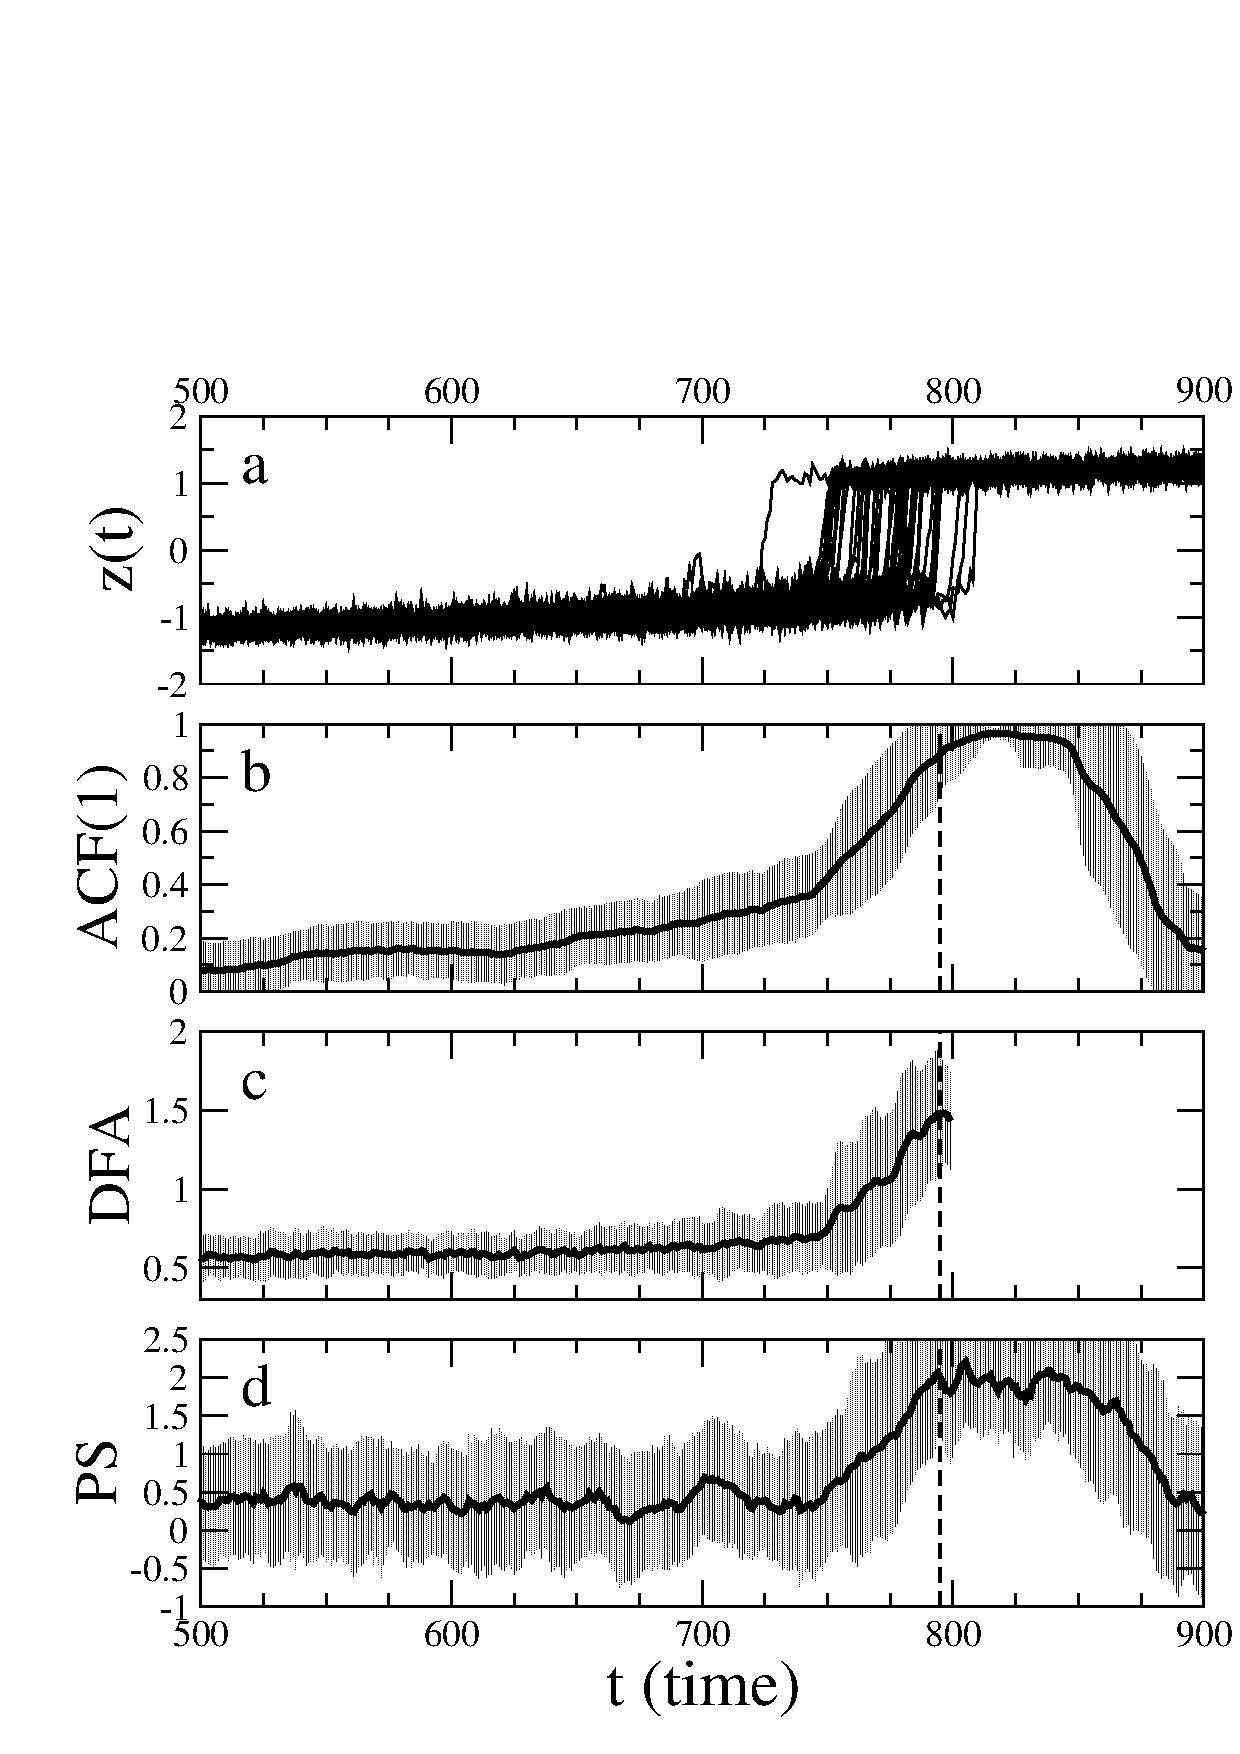
\includegraphics[width = \columnwidth]{newfigure}
\caption{ACF(1)-, DFA- and PS-indicators applied to model data. 
(a) Data from 50 runs of the saddle node bifurcation model (see equation \ref{saddlenode_eqn}).
(b,c,d) The mean ACF(1), DFA and PS-indicators (window size 100), with error bars of one standard deviation. The values of all the indicators begin to rise before the bifurcation, as expected, at around $t=750$, although it is most noticeable for the ACF(1)-indicator. Note also that the varience is much larger in the PS-indicator.\label{fig_new}}
\end{figure}

\end{document}


